%!TeX ts-program = xelatex
%!TeX encoding = utf-8 Unicode
\documentclass[ieeetran]{article}
\usepackage{amsmath, amssymb}
\usepackage{graphicx}

\title{Einführung in die Theoretische Informatik Aufgabenhandbuch}
\author{Efe Kamasoglu}

\begin{document}

\maketitle

\pagebreak


\section{Tutorium 1} % (fold)
\label{sec:tutorium_1}

\subsection{Beweistechniken für Sprachen} % (fold)
\label{sub:beweistechniken_für_sprachen}

\begin{itemize}
	\item $\mathbf{A \Longrightarrow B}$\textbf{:}
		\begin{enumerate}
			\item Annahme: $A$ ist wahr
			\item Zeige $B$ unter der Annahme
		\end{enumerate}
	\item $\mathbf{A \ gdw.\ B \ / \ A \iff B}$\textbf{:}
	 \begin{enumerate}
	   \item Zeige $A \Longleftarrow B$
	\item Zeige $A \Longrightarrow B$
			 \end{enumerate} 

\item \textbf{Beweis per Kontraposition für} $\mathbf{A \Longrightarrow B}$\textbf{:}
	\begin{enumerate}
		\item Zeige $\neg B \Longrightarrow \neg A$
	\end{enumerate}

\item \textbf{Beweis per Induktion für }$\mathbf{A \Longrightarrow A^n}$\textbf{:}
\begin{enumerate}
	\item Annahme: $A$
  \item Induktionsanfang: Zeige, dass $A^n$ für $n = 0$ gilt
  \item Induktionshypothese: $A^n$ gilt unter der Annahme für eine feste aber beliebige $n \in \mathbb{N}$
   
  \item Induktionsschritt: Zeige, dass $A^{n+1}$ unter der Annahme und der Hypothese gilt
\end{enumerate}

\item \textbf{Beweis durch Widerspruch für }$\mathbf{A}$\textbf{:}
	\begin{enumerate}
		\item Nehme an, dass $\neg A$ wahr ist
		\item Leite logische Konsequenzen aus dieser Annahme her
		\item Zeige, dass die Konsequenzen zum Widerspruch führen
	\end{enumerate}
\item \textbf{Widerlegen mithilfe eines Gegenbeispiels}
\end{itemize}


\section{Tutorium 2} % (fold)
\label{sec:tutorium_2}

\subsection{Strukturelle Induktion} % (fold)
\label{sub:strukturelle_induktion}
Um zu beweisen, dass eine Eigenschaft $P(r)$ für alle regulären Ausdrücke gilt.
\begin{enumerate}
	\item Zeige $P(\emptyset)$
	\item Zeige $P(\epsilon)$
	\item Zeige $P(a)$ für alle $a \in \Sigma$
	\item Unter der Annahme $P(\alpha)$ und $P(\beta)$ (I.H.), zeige $P(\alpha \beta)$ \\$\rightarrow$ verwende $L(\alpha \beta) =L(\alpha)L(\beta)$
	\item Unter der Annahme $P(\alpha)$ und $P(\beta)$ (I.H.), zeige $P(\alpha \ | \ \beta)$ \\$\rightarrow$ verwende $L(\alpha \ | \ \beta) =L(\alpha) \cup L(\beta)$
	\item Unter der Annahme $P(\alpha)$ (I.H.), zeige $P(\alpha^*)$ \\$\rightarrow$ verwende $L(\alpha^*) = L(\alpha)^*$
	
\end{enumerate}


\textit{\underline{Beispiel:}} $empty(r)$ entscheidet, ob $L(r) = \emptyset$. Zeige die Korrektheit der Konstruktion:

\begin{figure}[h!]
  \centering
  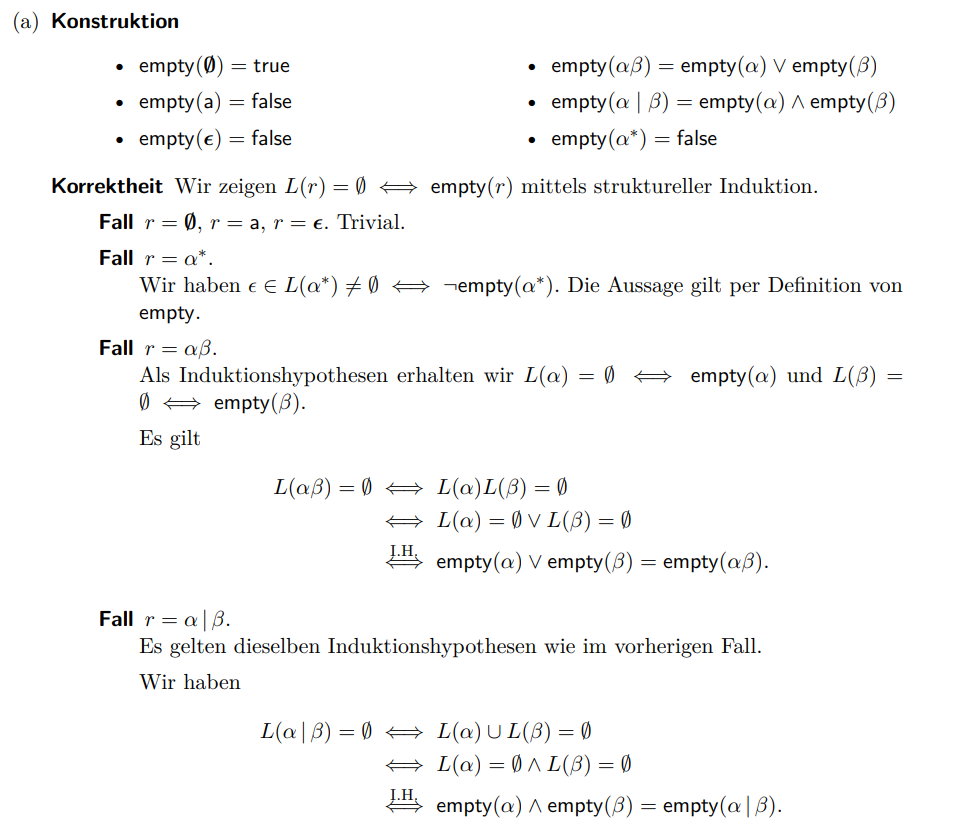
\includegraphics[width=1.0\linewidth]{strukturelleinduktion}
  \label{fig:strukturelleinduktion}
\end{figure}


\end{document}
